\documentclass[sigconf, anonymous]{acmart}

\newif\iftwocolumn
\newif\ifonecolumn
\twocolumntrue

\usepackage{preamble}

\fancyhf{} % Remove fancy page headers
\fancyhead[C]{Anonymous submission \#9999 to ACM CCS 2017} % TODO: replace 9999 with your paper number
\fancyfoot[C]{\thepage}

\setcopyright{none} % No copyright notice required for submissions
\acmConference[Anonymous Submission to ACM CCS 2018]{ACM Conference on Computer and Communications Security}{Due 8 May 2018}{Toronto, Canada}
\acmYear{2018}

\settopmatter{printacmref=false, printccs=true, printfolios=true} % We want page numbers on submissions

%%\ccsPaper{9999} % TODO: replace with your paper number once obtained

\begin{document}
\import{./}{title-text.tex}

\begin{abstract}
Open consensus protocols based on proof-of-work (PoW) mining are at the core of
cryptocurrencies such Bitcoin and Ethereum, as well as many others. In this
work, we construct a new primitive called
Non-Interactive-Proofs-of-Proof-of-Work (NIPoPoWs) that can be adapted into
existing PoW-based cryptocurrencies to improve their performance and extend
their functionality. Unlike a traditional blockchain client which must verify
the entire linearly-growing chain of PoWs, clients based on NIPoPoWs require
resources only logarithmic in the length of the blockchain. NIPoPoWs are thus
succinct proofs and require only a single message between the prover and the
verifier of the transaction.

With our construction we are able to prove a broad array of useful predicates in
the context of cross PoW-based blockchain transfers of assets,  including
predicates about facts buried deep within a blockchain which is necessary for
the basic application of accepting payments.

We provide empirical validation for NIPoPoWs through an implementation and
benchmark study, in the context of two new applications: First, we consider a
multi-client blockchain that supports all proof-of-work currencies rather than
just one, with up to 90\% reduction in bandwidth.  Second, we discuss a
``cross-chain ICO'' application that spans multiple independent blockchains.
Using our experimental data, we provide concrete parameters for our scheme.

\end{abstract}

\begin{CCSXML}
<ccs2012>
<concept>
<concept_id>10003752.10003777.10003789</concept_id>
<concept_desc>Theory of computation~Cryptographic protocols</concept_desc>
<concept_significance>500</concept_significance>
</concept>
</ccs2012>
\end{CCSXML}

\ccsdesc[500]{Theory of computation~Cryptographic protocols}
% -- end of section to replace with generated code

\keywords{proof-of-work; blockchain; non-interactive; SPV; cross-chain}

\maketitle

% \input{intro}
% \input{prelim}
% \input{definition}
% \section{Non-interactive blockchain \emph{suffix} proofs}
In this section, we modify the PoPoW scheme introduced in KLS~\cite{KLS} to make
it non-interactive. With foresight, we caution the reader that the
non-interactive construction we present in this section is \emph{insecure},
because the PoPoW scheme it is based on is also insecure. A very small patch
will later allow us to modify our construction to achieve security.

The previous work does not allow proving predicates about the blockchain, but
only allows determining if a block is part of an honest chain's suffix. In this
work, we allow provers to prove general predicates $Q$ about the chain $\chain$.
Among the predicates which are stable, in this section, we will limit ourselves
to \textit{suffix sensitive} predicates (similar to previous work in which the
verifier extracted the suffix adopted by an honest party, but not generic
predicates about it). We extend the protocol to support more flexible predicates
(such as transaction inclusion, as needed for our applications) which are not
limited to the suffix in Section~\ref{sec:infix}.

\begin{definition}[Suffix sensitivity]
A chain predicate $Q$ is called $k$-\emph{suffix sensitive} if its value
can be efficienty computed give the last $k$ blocks of the chain.
\end{definition}

\noindent\textbf{Example.}
In general our applications will require predicates that are not
suffix-sensitive. However, as an example, consider the predicate ``an Ethereum
contract at address $C$ has been initialized with code $h$ at least $k$ blocks
ago'' where $h$ does not invoke the \texttt{selfdestruct} opcode. This can be
implemented in a suffix-sensitive way because, in Ethereum, each block includes
a Merkle Trie over all of the contract codes~\cite{vitalik,wood}, which cannot be
changed after initialization. This predicate is thus also monotonic and
$k$-stable. Any predicate which is both \emph{suffix-sensitive} and
\emph{$k$-stable} must solely depend on data at block $\chain[-k]$.

\subsection{Construction}
We next present a generic form of the verifier first and the prover afterwards.
The generic form of the verifier works with any practical suffix proof protocol.
Therefore, we describe the generic verifier first before we talk about the
specific instantiation of our protocol. The generic verifier is given access to
call a protocol-specific proof comparison operator $\leq_m$ that we define. We
begin the description of our protocol by first illustrating the generic
verifier. Next, we describe the prover specific to our protocol. Finally, we
show the instantiation of the $\leq_m$ operator, which plugs into the generic
verifier to make a concrete verifier for our protocol.

\noindent{\bf The generic verifier.}
The \textsf{Verify} function of our NIPoPoW construction  for suffix predicates
is described in Algorithm~\ref{alg.nipopow-verifier}. The verifier algorithm is
parameterized by a chain predicate $Q$ and security parameters $k, m$; $k$
pertains to the amount of proof-of-work needed to bury a block so that it is
believed to remain stable (e.g., $k = 6$); $m$ is a security parameter
pertaining to the prefix of the proof, which connects the genesis block to the
$k$-sized suffix. The verifier receives several proofs by different provers in a
collection of proofs $\mathcal{P}$ at least one of which will be honest.
Iterating over these proofs, it extracts the best.

Each proof is a chain. For honest provers, these are subchains of the  adopted
chain. Proofs consist of two parts, $\pi$ and $\chi$; $\pi \chi$ must be a valid
chain; $\chi$ is the proof suffix; $\pi$ is the prefix. We require $|\chi| = k$.
For honest provers, $\chi$ is the last $k$ blocks of the adopted chain, while
$\pi$ consists of a selected subset of blocks from the rest of their chain
preceding $\chi$. The method of choice of this subset will become clear soon.

\import{./}{algorithms/alg.verifier-lite.tex}

The verifier compares the proof prefixes provided to it by calling the $\geq_m$
operator. We will get to the operator's definition shortly. Proofs are checked
for validity before comparison by ensuring $|\chi| = k$ and calling
$\mathsf{validChain}$ which checks if $\pi\chi$ is an anchored blockchain.

At each loop iteration, the verifier compares the next candidate proof prefix
$\pi$ against the currently best known proof prefix $\tilde\pi$ by calling $\pi
\geq_m \tilde\pi$. If the candidate prefix is better than the currently best
known proof prefix, then the currently known best prefix is updated by setting
$\tilde\pi \leftarrow \pi$. When the best known prefix is updated, the suffix
$\tilde\chi$ associated with the best known prefix is also updated to match the
suffix $\chi$ of the candidate proof by setting $\tilde\chi \leftarrow \chi$.
While $\tilde\chi$ is needed for the final predicate evaluation, it is not used
as part of any comparison, as it has the same size $k$ for all proofs. The best
known proof prefix is initially set to $(Gen)$, the trivial anchored chain
containing only the genesis block. Any well-formed proof compares favourably
against the trivial chain.

After the end of the \texttt{for} loop, the verifier will have determined the
best proof $(\tilde\pi, \tilde\chi)$. We will later prove that this proof will
necessarily belong to an honest prover with overwhelming probability. Since the
proof has been generated by an honest prover, it is associated with an
underlying honestly adopted chain $\chain$. The verifier then extracts the value
of the predicate $Q$ on the underlying chain. Note that, because the full chain
is not available to the verifier, the verifier here must evaluate the predicate
on the suffix. Because the predicate is suffix-sensitive, it is possible to do
so. As a technical detail, we denote $\tilde Q$ the predicate which accepts only
a $k$-suffix of a blockchain and outputs the same value that $Q$ would have
output if it had been evaluated on a chain with that suffix.

\import{./}{algorithms/alg.nipopow-prover.tex}

\noindent
\textbf{The concrete prover.}
The NIPoPoW prover construction is shown in Algorithm~\ref{alg.nipopow-prover}.
The honest prover is supplied with an honestly adopted chain $\chain$ and
security parameters $m, k, \delta$ and returns proof $\pi\chi$, which is a
chain. The suffix $\chi$ is the last $k$ blocks of $\chain$. The prefix $\pi$ is
constructed by selecting various blocks from $\chain[:-k]$ and adding them to
$\pi$, which consists of a number of blocks for every level $\mu$ from the
highest level $|\chain[-k].\textsf{interlink}|$ down to $0$. At the highest
possible level at which at least $m$ blocks exist, all these blocks are
included. Then, inductively, for every superchain of level $\mu$ that is
included in the proof, the suffix of length $m$ is taken. Then the underlying
superchain of level $\mu - 1$ spanning from this suffix until the end of the
blockchain is also included. All the $\mu$-superblocks which are within this
range of $m$ blocks will also be $(\mu-1)$-superblocks and so we do not want to
keep them in the proof twice (we use the union set notation to indicate this).
Each underlying superchain will have $2m$ blocks in expectation and always at
least $m$ blocks. This is repeated until level $\mu = 0$ is reached. Note that
no check is necessary to make sure the top-most level has at least $m$ blocks,
even though the verifier requires this. The reason is the following: Assume the
blockchain has at least $m$ blocks in total. Then, when a superchain of level
$\mu$ has less than $m$ blocks in total, these blocks will all be necessarily
included into the proof by a lower-level superchain $\mu - i$ for some $i > 0$.
Therefore, it does not hurt to add them to $\pi$ earlier.

Figure~\ref{fig.nipopow} contains an example proof constructed for parameters
$m = k = 3$. The top superchain level which contains at least $m$ blocks is
level $\mu = 2$. For the $m$-sized suffix of that level, $6$ blocks of
superblock level $1$ are included to span the same range ($2m$ blocks at this
level). For the last $3$ blocks of the $1$-superchain, blocks of level $0$
spanning the same range are included (again $2m$ blocks at this level). Note
that the superchain at a lower levels may reach closer to the end of the
blockchain than a higher level. Level $3$ was not used, as it does not yet have
a sufficient number of blocks.

\begin{figure}[h]
    \caption{
    NIPoPoW \emph{prefix} $\pi$ for $m = 3$. It includes the Genesis block $G$,
    three $2$-superblocks, six $1$-superblocks, and six $0$-blocks.
    }
    \centering
    \iftwocolumn
        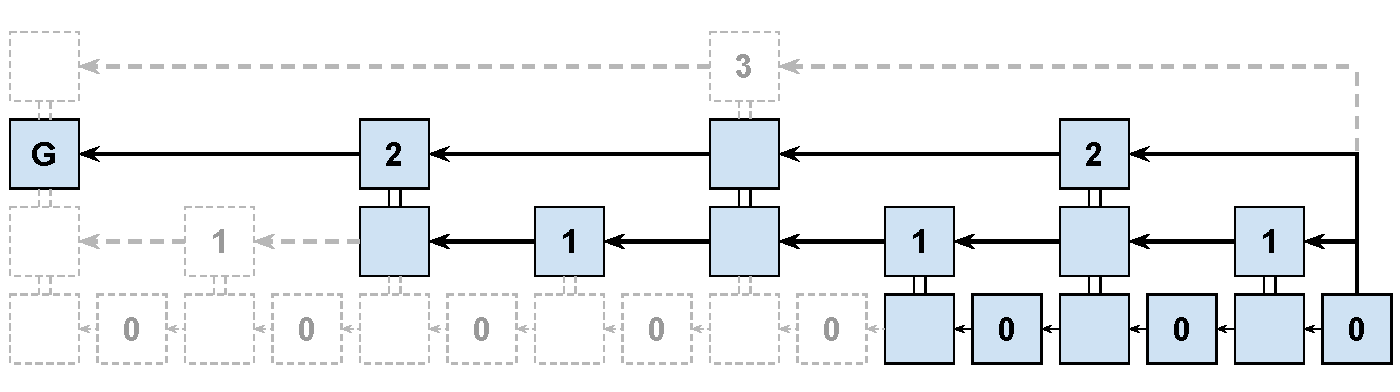
\includegraphics[width=0.9\columnwidth,keepaspectratio]{figures/non-interactive-popow.pdf}
    \else
        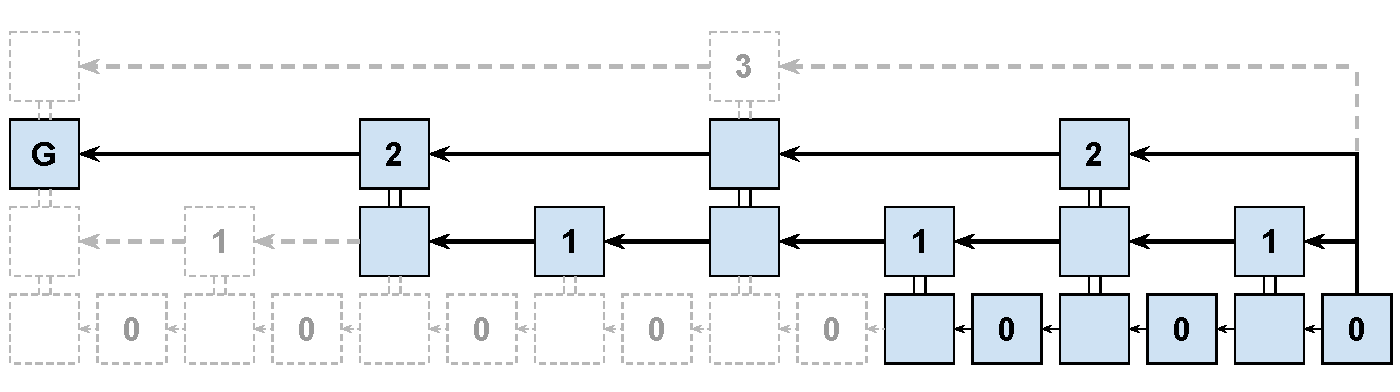
\includegraphics[width=0.7\columnwidth,keepaspectratio]{figures/non-interactive-popow.pdf}
    \fi
    \label{fig.nipopow}
\end{figure}

\noindent
\textbf{The concrete verifier.}
The $\geq_m$ operator which performs the comparison of proofs is presented in
Algorithm~\ref{alg.nipopow-maxchain}. It takes proofs $\pi_A$ and $\pi_B$ and
returns \emph{true} if the first proof is winning, or \emph{false} if the second
is winning. It first computes the LCA block $b$ between the proofs. As parties
$A$ and $B$ agree that the blockchain is the same up to block $b$, arguments
will then be taken for the diverging chains after $b$. An \emph{argument} is a
subchain of a proof provided by a prover such that its blocks are after the LCA
block $b$ and they are all at the same level $\mu$. The best possible argument
from each player's proof is extracted by calling the $\text{best-arg}_m$
function.
% We call the willingness of the verifier to allow each prover to be
% evaluated based on their best argument the \textit{principle of charity}.
To find the best argument of a proof $\pi$ given $b$, $\text{best-arg}_m$
collects all the indices $\mu$ which point to superblock levels that contain
valid arguments after block $b$. Argument validity requires that there are at
least $m$ $\mu$-superblocks following block $b$, which is captured by the
comparison $|\pi\upchain^\mu\{b:\}| \geq m$. $0$ is always considered a valid
level, regardless of how many blocks are present there. These level indices are
collected into set $M$. For each of these levels, the score of their respective
argument is evaluated by weighting the number of blocks by the level as
$2^\mu|\pi\upchain^\mu\{b:\}|$. The highest possible score across all levels is
returned. Once the score of the best argument of both $A$ and $B$ is known, they
are directly compared and the winner returned.  An advantage is given to the
first proof in case of a tie by making the $\geq_m$ operator favour the
adversary $\mathcal{A}$.

\import{./}{algorithms/alg.nipopow-maxchain.tex}

Looking ahead, the core of the security argument will be that, given a block
$b$, it will be difficult for a mining minority adversary to produce blocks
descending from $b$ faster than the honest party. This holds for blocks of any
level.

% \input{other}
% \input{analysis}

\import{./}{nipopows-body.tex}

\newpage

\appendix
\section*{Appendix}

% \section{Backbone integration}
% \label{sec.appendix-backbone}
%
% %We use this model to explore which predicates are reliable and can be proven
% %succinctly.
%
% In this section, we illustrate the detailed formalisms to integrate our proof
% systems with the backbone model \cite{backbone}.
%
% The backbone protocol of a miner node is shown in Algorithm~\ref{alg.backbone}.
% The honest miner maintains the longest chain from the network and tries to mine
% on top of it. In Algorithm~\ref{alg.backbone-prover}, we illustrate our new
% entity for the model, the full node or \textit{prover}.  While the full node is
% not mining, it maintains a state with the longest chain from the network.
% Furthermore, whenever it is asked to prove a predicate $Q$ about its local
% chain $\chain$, it calls a Prove function to provide the proof.  We leave this
% Prove function undefined here, as it is part of the concrete protocol
% construction. On the other hand, in Algorithm~\ref{alg.generic-verifier} we
% illustrate another new entity to the model, the generic \textit{verifier},
% which is stateless, but receives proofs from the provers on the network (via
% the environment) and takes a decision about a predicate on the blockchain it
% believes to be the longest.
%
% \import{./}{algorithms/alg.backbone.tex}
% \import{./}{algorithms/alg.backbone-prover.tex}
% \import{./}{algorithms/alg.verifier-framework.tex}
%
% The prover which additionally maintains the \textit{blockById},
% \textit{depth} and \textit{realLink} data structures is illustrated in
% Algorithm~\ref{alg.backbone-velvet-prover}.
%
% \import{./}{algorithms/alg.backbone-velvet-prover.tex}

% \noindent
% \textbf{Analysis of the attack.}

% \noindent
% \textbf{Interlink optimizations.}
% \noindent
% \textbf{Proof of security. }
% \noindent
% \textbf{Full proofs. }

\section{Velvet forks revisited}

\import{./}{algorithms/alg.nipopow-velvet-innerchain.tex}

For completeness, we include the necessary changes needed in the various
construction algorithms in order to support a velvet fork. These are shown in
Algorithm~\ref{alg.nipopow-velvet-innerchain},
Algorithm~\ref{alg.nipopow-velvet-follow}, and
Algorithm~\ref{alg.nipopow-velvet-prover}.
Algorithm~\ref{alg.nipopow-velvet-innerchain} defines the innerChain method,
which replaces the upchain/downchain abstraction that can be easily used in a
fully upgraded chain.

The following theorem establishes the security of NIPoPoWs in velvet forks.

\restateThmVelvetSuccinctness*
\import{./}{proofs/velvetsuccinctness.tex}

\import{./}{algorithms/alg.nipopow-velvet-follow.tex}
\import{./}{algorithms/alg.nipopow-velvet-prover.tex}

\import{./}{security-full.tex}
\import{./}{attack-full.tex}
\import{./}{infix-full.tex}

% \section{Full proofs}
%
% \label{sec.proofs}
% \restateThmPredicatePersistence*
% \import{./}{proofs/predicatepersistence.tex}
% \noindent
% \textbf{Theorem~\ref{thm.few-levels}}
% \restateThmFewLevels*
% \import{./}{proofs/fewlevels.tex}
% \noindent
% \textbf{Theorem~\ref{thm.large-expansion}}
% \restateThmLargeExpansion*
% \import{./}{proofs/largeexpansion.tex}
% \noindent
% \textbf{Lemma~\ref{lem.small-support}}
% \restateThmSmallSupport*
% \import{./}{proofs/smallsupport.tex}
% \noindent
% \textbf{Theorem~\ref{thm.succinctness}}
% \restateThmSuccinctness*
% \import{./}{proofs/succinctness.tex}
% \noindent
% \textbf{Theorem~\ref{thm.infix-security}}
% \restateThmInfixSecurity*
% \import{./}{proofs/infixsecurity.tex}
% \noindent
% \textbf{Theorem~\ref{thm.velvet-succinctness}}


% %\input{app-ouroboros}
% \input{app-validator}
% \input{app-other}
% \input{app-proofs}
% \input{app-construction}

\bibliographystyle{ACM-Reference-Format}
% \bibliography{pubs,abbrev3,crypto}
\bibliography{bibliography}

\end{document}
